\documentclass[11pt]{article}
    \title{\textbf{Math 217 Homework I}}
    \author{Khac Nguyen Nguyen}
    \date{}

    \addtolength{\topmargin}{-3cm}
    \addtolength{\textheight}{3cm}

\usepackage{amsmath}
\usepackage{mathtools}
\usepackage{amsthm}
\usepackage{amssymb}
\usepackage{pgfplots}
\usepackage{xfrac}
\usepackage{hyperref}
\usepackage{graphicx}

\usepgfplotslibrary{polar}
\usepgflibrary{shapes.geometric}
\usetikzlibrary{calc}
\pgfplotsset{compat = newest}
\pgfplotsset{my style/.append style = {axis x line = middle, axis y line = middle, xlabel={$x$}, ylabel={$y$}, axis equal}}
\begin{document}
\section{}
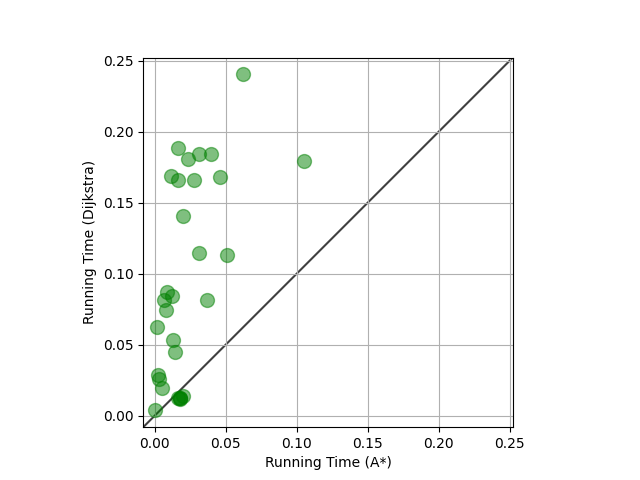
\includegraphics[scale = 0.8]{running_time.png}
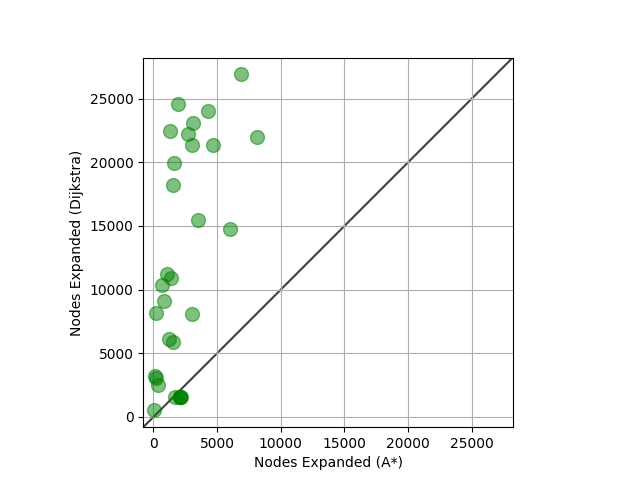
\includegraphics[scale = 0.8]{nodes_expanded.png}
\subsection*{a.}
A* is a faster version of dijkstra because it use 
BFS and the heuristic function to speed the process up. \\
\subsection*{b.}
The point are in the same relative location in the two spots 
because the number of nodes expanded and the running time are inter-dependent 
and hence increase at the same rate.
\section{}
In the plot, we can see that dijkstra always run twice as fast as WA*, which is the same as $W$.
Hence, there is a high chance that they are implementing Dijkstra the wrong way, 
that is they are simply multiplying the cost by 2

\end{document}